\حصہ{ریمان مجموعے اور قطعی تکملات}
گزشتہ حصے میں ہم نے فاصلے، رقبے، حجم اور اوسط قیمتوں کو متناہی مجموعوں کی مدد سے حاصل کیا۔ منتخب تفاعل کی قیمتوں کو وقفوں کی لمبائیوں کے ساتھ ضرب دیتے ہوئے یہ مجموعے حاصل کیے گئے۔اس حصہ میں  ان وقفوں کی لمبائیوں کو کم سے کم اور تعداد کو زیادہ سے زیادہ کرتے ہوئے  مجموعہ کی تحدیدی قیمت پر غور کیا جائے گا۔ متعدد ارکان پر مشتمل مجموعے کو ظاہر کرنے کی علامت پہلے متعارف کرتے ہیں۔

\جزوحصہء{متناہی مجموعہ کی علامت}
درج ذیل مجموعہ کو
\begin{align*}
f(t_1)\Delta t+f(t_2)\Delta t+\cdots+f(t_n)\Delta t
\end{align*}
یونانی حروف تہجی کا بڑا حرف \عددی{\Sigma} ("سگما") استعمال کرتے ہوئے  \عددی{\sum_{k=1}^{n}f(t_k)\Delta t} سے ظاہر کیا جاتا ہے جو \عددی{k} کی \عددی{1} تا \عددی{n} قیمتوں کے لئے \عددی{\Delta t} ضرب \عددی{t_k} پر \عددی{f} کی قیمتوں کا مجموعہ ہے۔ مجموعہ کی یوں اظہار  کو سگما علامتی اظہار کہتے ہیں۔ 

\ابتدا{تعریف}\موٹا{متناہی مجموعہ کا سگما علامتی اظہار}\\
علامت \عددی{\sum_{k=1}^{n}a_k} سے مراد مجموعہ \عددی{a_1+a_2+\cdots+a_n} ہے۔مجموعہ کے \اصطلاح{ارکان}\فرہنگ{مجموعہ!ارکان}\حاشیہب{terms}\فرہنگ{terms} \عددی{a_1} تا \عددی{a_n} ہیں جہاں \عددی{a_1} مجموعے کا پہلا اور \عددی{a_n}  مجموعے کا آخری رکن ہے۔ متغیر \عددی{k} \اصطلاح{مجموعی سلسلہ کا اشاری}\فرہنگ{مجموعی سلسلہ!اشاری}\حاشیہب{index of summation}\فرہنگ{index!summation} کہلاتا ہے۔ \عددی{k} کی قیمتیں \عددی{1} تا \عددی{n} عدد صحیح ہیں۔ \اصطلاح{مجموعی سلسلہ کا زیریں حد}\فرہنگ{مجموعی سلسلہ!زیریں حد}\حاشیہب{lower limit of summation}\فرہنگ{summation!lower limit} \عددی{1} جبکہ \اصطلاح{مجموعی سلسلہ کا بالائی حد}\فرہنگ{مجموعی سلسلہ!بالائی حد}\حاشیہب{upper limit of summation}\فرہنگ{summation!upper limit} \عددی{n} ہے۔زیریں اور بالائی حدود کوئی بھی دو عدد صحیح ممکن ہیں۔
\انتہا{تعریف}
%=====================

\ابتدا{مثال}
\begin{align*}
\begin{array}{lcc}
\text{\RL{مجموعہ کی سگما صورت}}&\text{\RL{ارکان کی صورت میں مجموعہ}}&\text{\RL{مجموعہ کی قیمت}}\\
\toprule
\sum\limits_{k=1}^{5}k&1+2+3+4+5&15\\
\sum\limits_{k=1}^{3}(-1)^kk&(-1)^1(1)+(-1)^2(2)+(-1)^3(3)&-1+2-3=-2\\
\sum\limits_{k=1}^{2}\frac{k}{k+1}&\frac{1}{1+1}+\frac{2}{2+1}&\frac{1}{2}+\frac{2}{3}=\frac{7}{6}
\end{array}
\end{align*}
\انتہا{مثال}

مجموعی سلسلہ کا زیریں حد \عددی{1} سے ہٹ کر ہو سکتا ہے۔ 

\ابتدا{مثال}
مجموعہ \عددی{1+3+5+7+9} کو سگما علامتی روپ میں لکھیں۔

حل:\quad
\begin{align*}
&\sum\limits_{k=0}^{4} (2k+1)&&\text{\RL{$k=0$ سے شروع کیا گیا ہے}}\\
&\sum\limits_{k=1}^{5} (2k-1)&&\text{\RL{$k=1$ سے شروع کیا گیا ہے}}
\end{align*}
\انتہا{مثال}
%============================

\جزوحصہء{متناہی مجموعہ کا الجبرا}
متناہی مجموعوں کے ساتھ کام کرتے ہوئے درج ذیل قواعد بروئے کار لائے جا سکتے ہیں۔
\begin{description}
\item{قاعدہ مجموعہ:}\quad 
$\sum\limits_{k=1}^n (a_k+b_k)=\sum\limits_{k=1}^na_k+\sum\limits_{k=1}^nb_k$
\item{قاعدہ فرق:}\quad
$\sum\limits_{k=1}^n (a_k-b_k)=\sum\limits_{k=1}^na_k-\sum\limits_{k=1}^nb_k$
\item{قاعدہ ضرب مستقل:}\quad
$\sum\limits_{k=1}^nca_k=c\cdot\sum_{k=1}^na_k$
جہاں \عددی{c} کوئی عدد ہے۔
\item{قاعدہ مستقل قیمت:}\quad
$\sum\limits_{k=1}^nc=n\cdot c$
جہاں \عددی{c} کوئی مستقل قیمت ہے۔
\end{description}

اس فہرست میں کوئی حیران کن حقیقت پیش نہیں کی گئی ہے۔ ان کے با ضابطہ ثبوت (الکراجی) الجبرائی ماخوذ سے حاصل کیے جا سکتے ہیں جنہیں  ضمیمہ \حوالہ{ضمیمہ_الف} میں پیش کیا گیا ہے۔

\ابتدا{مثال}
\begin{align*}
&\sum\limits_{k=1}^n(3k-k^2)=3\sum\limits_{k=1}^nk-\sum\limits_{k=1}^nk^2&&\text{\RL{قاعدہ فرق اور قاعدہ ضرب مستقل}}\\
&\sum\limits_{k=1}^n(-a_k)=\sum\limits_{k=1}^n(-1)\cdot a_k=-1\cdot\sum\limits_{k=1}^na_k=-\sum\limits_{k=1}^na_k&&\text{\RL{قاعدہ ضرب مستقل}}\\
&\sum\limits_{k=1}^3(k+4)=\sum\limits_{k=1}^3k+\sum\limits_{k=1}^34\\
&\quad\quad\quad\quad\quad=(1+2+3)+(3\cdot 4)&&\text{\RL{قاعدہ مستقل قیمت}}\\
&\quad\quad\quad\quad\quad=6+12=18
\end{align*}
\انتہا{مثال}
%=====================
\جزوحصہء{مثبت عدد صحیح کے کلیات مجموعہ}
متناہی مجموعوں کے کئی کلیات پائے جاتے ہیں جن میں سے مشہور ترین کلیات شروع کے \عددی{n} عدد صحیح کا مجموعہ ہے (جو گاوس نے \عددی{5} سال کی عمر میں اخذ کیا) اور شروع کے \عددی{n} عدد صحیح کے مربع اور مکعب کے مجموعوں کے کلیات ہیں۔
\begin{gather}
\begin{aligned}\label{مساوات_تکمل_قاعدہ_عدد_صحیح_مجموعہ}
\sum\limits_{k=1}^nk&=\frac{n(n+1)}{2}&&\text{\RL{ابتدائی $n$ عدد صحیح}}\\
\sum\limits_{k=1}^nk^2&=\frac{n(n+1)(2n+1)}{6}&&\text{\RL{ابتدائی $n$ عدد صحیح کے مربع}}\\
\sum\limits_{k=1}^nk^3&=\big(\frac{n(n+1)}{2}\big)^2&&\text{\RL{ابتدائی $n$ عدد صحیح کے مکعب}}
\end{aligned}
\end{gather}
\ابتدا{مثال}
\عددی{\sum_{k=1}^4(k^2-3k)} تلاش کریں۔

حل:\quad
ہم مجموعہ کو مجموعی سلسلہ کے روپ میں لکھے بغیر الجبرائی قواعد استعمال کرتے ہوئے جواب حاصل کرتے ہیں۔
\begin{align*}
\sum\limits_{k=1}^4(k^2-3k)&=\sum\limits_{k=1}^4k^2-3\sum\limits_{k=1}^4k&&\text{\RL{قاعدہ فرق اور قاعدہ ضرب مستقل}}\\
&=\frac{4(4+1)(8+1)}{6}-3\big(\frac{4(4+1)}{2}\big)&&\text{\RL{$n=4$ لیتے ہوئے مساوات \حوالہ{مساوات_تکمل_قاعدہ_عدد_صحیح_مجموعہ}}}\\
&=30-30=0
\end{align*} 
\انتہا{مثال}
%====================
\begin{figure}
\centering
\begin{tikzpicture}[font=\small,declare function={f(\x)=-sin(deg(\x))-1/6*(\x/pi)^2*sin(deg(3*\x));}]
\pgfmathsetmacro{\ca}{0.5}
\pgfmathsetmacro{\cb}{1.5}
\pgfmathsetmacro{\cc}{2.5}
\pgfmathsetmacro{\cd}{2.9}
\pgfmathsetmacro{\ce}{3.7}
\pgfmathsetmacro{\cf}{4.3}
\pgfmathsetmacro{\cg}{5}
\pgfmathsetmacro{\ch}{5.5}
\pgfmathsetmacro{\xa}{1}
\pgfmathsetmacro{\xb}{2}
\pgfmathsetmacro{\xc}{2.8}
\pgfmathsetmacro{\xd}{3.4}
\pgfmathsetmacro{\xe}{4.2}
\pgfmathsetmacro{\xf}{4.8}
\pgfmathsetmacro{\xg}{5.2}
\pgfmathsetmacro{\xh}{6}
\pgfmathsetmacro{\pa}{f(\ca)}
\pgfmathsetmacro{\pb}{f(\cb)}
\pgfmathsetmacro{\pc}{f(\cc)}
\pgfmathsetmacro{\pd}{f(\cd)}
\pgfmathsetmacro{\pe}{f(\ce)}
\pgfmathsetmacro{\pf}{f(\cf)}
\pgfmathsetmacro{\pg}{f(\cg)}
\pgfmathsetmacro{\ph}{f(\ch)}
\begin{axis}[clip=false,width=0.75*\textwidth,height=6cm,font=\scriptsize,axis lines=middle,xmin=0,xtick={\empty},ytick={\empty},xmax=7,xlabel={$x$},ylabel={$y$},xlabel style={at={(current axis.right of origin)},anchor=west},ylabel style={at={(current axis.above origin)},anchor=south}]
\addplot[domain=0.2:6.2,smooth]{f(x)};
\draw(axis cs:\ca,0)node[circ]{}node[above]{$c_1$}node[below left]{$x_0=a$}--(axis cs:\ca,\pa)node[circ]{}node[below left]{$(c_1,f(c_1))$};
\draw(axis cs:\cb,0)node[circ]{}node[above]{$c_2$}--(axis cs:\cb,\pb)node[circ]{}node[below]{$(c_2,f(c_2))$};
\draw[dashed](axis cs:\ca,\pa)--(axis cs:\xa,\pa);
\draw[dashed](axis cs:\xa,0)node[below left]{$x_1$}--(axis cs:\xa,\pb)--(axis cs:\xb,\pb)--(axis cs:\xb,0)node[below left]{$x_2$};
\draw[dashed](axis cs:\xb,\pc)--(axis cs:\xc,\pc)--(axis cs:\xc,0);
\draw[dashed](axis cs:\xc,\pd)--(axis cs:\xd,\pd)--(axis cs:\xd,0)node[below,fill=white]{$x_{k-1}$};
\draw[dashed](axis cs:\xd,0)--(axis cs:\xd,\pe)--(axis cs:\xe,\pe);
\draw(axis cs:\ce,0)node[circ]{}node[above right]{$c_k$}--(axis cs:\ce,\pe)node[circ]{}node[above left]{$(c_k,f(c_k))$};
\draw[dashed](axis cs:\xe,0)node[below,fill=white]{$x_k$}--(axis cs:\xe,\pf)--(axis cs:\xf,\pf)--(axis cs:\xf,0);
\draw[dashed](axis cs:\xf,\pg)--(axis cs:\xg,\pg)--(axis cs:\xg,0)node[below]{$x_{n-1}$};
\draw[dashed](axis cs:\xg,\pg)--(axis cs:\xg,\ph)--(axis cs:\xh,\ph)--(axis cs:\xh,0)node[below right,xshift=-2mm]{$x_n=b$};
\draw(axis cs:\ch,0)node[circ]{}node[above right]{$c_n$}--(axis cs:\ch,\ph)node[circ]{}node[above]{$(c_n,f(c_n))$};
\draw(axis cs:1.5,0.5)node[]{$y=f(x)$};
\end{axis}
\end{tikzpicture}
\caption{بند وقفہ \عددی{[a,b]} پر عمومی تفاعل \عددی{y=f(x)}۔ تفاعل اور \عددی{x} محور کے بیچ رقبہ کو تخمینی طور پر مستطیلوں سے ظاہر کیا گیا ہے۔ نقطہ \عددی{c_1} کو عین \عددی{x_0} پر منتخب کیا ہوا دکھایا گیا ہے۔}
\label{شکل_تکمل_رقبہ_بذریعہ_مستطیل_الف}
\end{figure}
\جزوحصہء{ریمان مجموعے}
ہم نے حصہ \حوالہ{حصہ_تکمل_اندازہ_بذریعہ_متناہی_مجموعہ} میں تخمینی مجموعوں پر غور کیا جو زیادہ عمومی \اصطلاح{ریمان مجموعہ} کی مخصوص مثالیں تھیں۔ ان مثالوں میں تفاعل کی قیمتیں غیر منفی تھیں جبکہ ریمان مجموعہ میں ایسی پابندی نہیں پائی جاتی ہے۔ وقفہ \عددی{[a,b]} پر دیے گئے اختیاری استمراری تفاعل \عددی{y=f(x)} کو \عددی{a} اور \عددی{b} کے بیچ نقاط \عددی{x_1,x_2,\cdots,x_{n+1}} پر \عددی{n} ذیلی وقفوں میں تقسیم کیا جاتا ہے (شکل \حوالہ{شکل_تکمل_رقبہ_بذریعہ_مستطیل_الف})۔یہ نقطے صرف درج ذیل شرط کے تحت منتخب کیے جاتے ہیں۔
\begin{align*}
a<x_1<x_2<\cdots<x_{n-1}<b
\end{align*}
اس علامتی روپ میں مطابقت پیدا کرنے کی خاطر \عددی{a} کو \عددی{x_0} اور \عددی{b} کو \عددی{x_n} سے ظاہر کیا جاتا ہے۔ درج ذیل سلسلہ
\begin{align*}
P=\{x_0,x_1,\cdots,x_n \}
\end{align*}
کو \عددی{[a,b]} کی \اصطلاح{خانہ بندی}\فرہنگ{خانہ بندی}\حاشیہب{partition}\فرہنگ{partition} کہتے ہیں۔

\عددی{P} کی خانہ بندی درج ذیل \عددی{n} عدد بند \اصطلاح{ذیلی وقفوں}\فرہنگ{وقفہ!ذیلی}\حاشیہب{subintervals}\فرہنگ{subintervals} کو ظاہر کرتی ہے۔
\begin{align*}
[x_0,x_1],[x_1,x_2],\cdots,[x_{n-1},x_n]
\end{align*}
بند ذیلی وقفہ \عددی{[x_{k-1},x_k]} کو \عددی{P} کا \عددی{k} واں ذیلی وقفہ کہتے ہیں۔\\
\begin{center}
\begin{tikzpicture}
\draw[-latex](-0.25,0)--(8.75,0)node[right]{$x$};
\foreach \x/\s in {0/x_0=a,1/x_1,1.75/x_2,3.2/x_{k-1},4.95/x_k,6.7/x_{n-1},8/x_{n}=b}{\draw(\x,-0.1)node[below]{$\s$}--++(0,0.2);}
\draw[thick](3.2,0)--(4.95,0)node[pos=0.5,above]{\RL{\عددی{k} واں ذیلی وقفہ}};
\draw(2.38,-0.1)node[below]{$\cdots$};
\draw(5.825,-0.1)node[below]{$\cdots$};
\end{tikzpicture}
\end{center}
\عددی{k} ویں ذیلی وقفہ کی لمبائی \عددی{\Delta x_k=x_k-x_{k-1}} ہے۔
\begin{center}
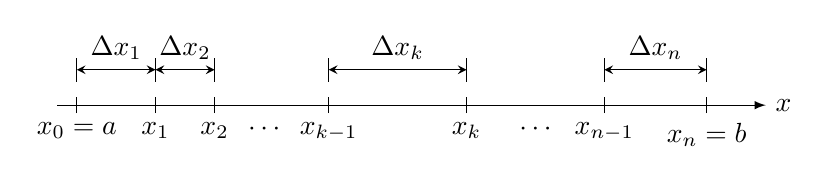
\begin{tikzpicture}
\draw[-latex](-0.25,0)--(8.75,0)node[right]{$x$};
\foreach \x/\s in {0/x_0=a,1/x_1,1.75/x_2,3.2/x_{k-1},4.95/x_k,6.7/x_{n-1},8/x_{n}=b}{\draw(\x,-0.1)node[below]{$\s$}--++(0,0.2); \draw(\x,0.3)--++(0,0.3);}
\draw(2.38,-0.1)node[below]{$\cdots$};
\draw(5.825,-0.1)node[below]{$\cdots$};
\foreach \xa/\xb/\s in {0/1/1,1/1.75/2,3.2/4.95/k,6.7/8/n}{\draw[stealth-stealth](\xa,0.45)--(\xb,0.45)node[pos=0.5,above]{$\Delta x_{\s}$};}
\end{tikzpicture}
\end{center}
ہر ذیلی وقفہ \عددی{[x_{k-1},x_k]} میں ہم کوئی نقطہ \عددی{c_k} منتخب کرتے ہوئے ذیلی وقفہ میں تفاعل \عددی{y=f(x)} پر نقطہ \عددی{(c_k,f(c_k))} تک مستطیل بناتے ہیں۔ جب تک نقطہ \عددی{c_k} ذیلی وقفہ \عددی{[x_{k-1},x_k]} میں پایا جاتا ہو اس کا مقام غیر اہم ہے (شکل \حوالہ{شکل_تکمل_رقبہ_بذریعہ_مستطیل_الف})۔

اگر \عددی{f(c_k)} مثبت ہو تب عدد \عددی{f(c_k)\Delta x_k} مستطیل کے قد ضرب قاعدہ یعنی مستطیل کے رقبہ کے برابر ہو گا۔ اگر \عددی{f(c_k)} منفی عدد ہو تب \عددی{f(c_k)\Delta x_k} مستطیل کے رقبہ کے نفی کے برابر ہو گا۔ ہم ان تمام \عددی{f(c_k)\Delta x_k} حاصل ضرب جن کی تعداد \عددی{n} ہے کا مجموعہ لیتے ہیں۔
\begin{align*}
S_P=\sum\limits_{k=1}^nf(c_k)\Delta x_k
\end{align*}
یہ مجموعہ جو \عددی{P} اور \عددی{c_k} کی انتخاب پر منحصر ہے وقفہ \عددی{[a,b]} پر \عددی{f} کا \اصطلاح{ریمان مجموعہ}\فرہنگ{ریمان!مجموعہ}\حاشیہب{Riemann sum}\فرہنگ{Riemann!sum} کہلاتا\حاشیہد{جرمنی کے ریاضی دان برنہارڈ ریمان [1826-1866] نے ایسے مجموعوں کی تحدیدی قیمتوں پر کام کیا۔} ہے۔

\عددی{[a,b]} کے خانوں کی چوڑائی کم سے کم کرتے ہوئے خانہ بندی سے حاصل مستطیل تفاعل \عددی{f} اور \عددی{x} محور کے بیچ خطہ کو بہتر سے بہتر  ظاہر کرتے ہیں۔یوں ہم توقع کرتے ہیں کہ ریمان مجموعہ کی تحدیدی  قیمت پائی جائے گی۔ ہماری اس توقع کو پرکھنے کی خاطر ہمیں خانوں کی چوڑائی کم سے کم کرنے کو ریاضیاتی صورت میں لکھنا ہو گا اور جاننا ہو گا کہ آیا مطابقتی مجموعہ کی کوئی تحدیدی قیمت پائی جاتی ہے۔ ہم درج ذیل تعریف کی مدد سے ایسا کر پائیں گے۔

خانہ بندی \عددی{P} کی \اصطلاح{معیار}\فرہنگ{معیار}\حاشیہب{norm}\فرہنگ{norm} سے مراد سب سے لمبے خانے کی لمبائی ہے جس کو درج ذیل علامت سے ظاہر کیا جاتا ہے۔
\begin{align*}
&\norm{P} &&\text{\RL{(اس کو "$P$ کا معیار" پڑھیں)}}
\end{align*}
خانوں کی چوڑائی کم سے کم کرنے  کی بجائے اب ہم کہتے ہیں کہ خانوں کی معیار صفر تک پہنچائی جاتی ہے۔جیسے جیسے معیار کی قیمت صفر کے نزدیک ہوتی جاتی ہے ویسے ویسے ذیلی وقفوں کی لمبائی کم سے کم اور ان کی تعداد زیادہ سے زیادہ ہوتی جاتی ہے۔ خانوں کی چوڑائی کم کرنے سے باریک مستطیل پیدا ہوں گے۔

\ابتدا{مثال}
وقفہ \عددی{[0,2]} کی خانہ بندی  سلسلہ \عددی{P=\{0,0.2,0.6,1,1.5,2\}} ہے۔ \عددی{P} کے  پانچ ذیلی وقفے درج ذیل ہیں۔
\begin{align*}
[0,0.2],\,[0.2,0.6],\,[0.6,1],\,[1,1.5],\,[1.5,2]
\end{align*} 
ان ذیلی وقفوں کی لمبائیاں \عددی{\Delta x_1=0.2}، \عددی{\Delta x_2=0.4}، \عددی{\Delta x_3=0.4}، \عددی{\Delta x_4=0.5} اور \عددی{\Delta x_5=0.5} ہیں۔ ان میں سب سے لمبے ذیلی وقفہ کی لمبائی \عددی{0.5} ہے لہٰذا خانہ بندی \عددی{P} کا معیار \عددی{\norm{P}=0.5} ہے۔ اس مثال میں دو ذیلی وقفوں کی لمبائی \عددی{0.5} ہے۔
\انتہا{مثال}
%===========================

\ابتدا{تعریف}\موٹا{قطعی تکمل بطور ریمان مجموعوں کا حد}\\

\انتہا{تعریف}

